\documentclass[aspectratio=169,10pt]{beamer}

% -------------------------------------------------
% Theme and typography
% -------------------------------------------------
\usetheme[progressbar=frametitle,numbering=fraction]{metropolis}
\usefonttheme{professionalfonts}

\usepackage[T1]{fontenc}
\usepackage{lmodern}
\usepackage{amsmath,amssymb,mathtools}
\usepackage{booktabs}
\usepackage{array}
\usepackage{tikz}
\usetikzlibrary{automata,positioning,arrows.meta,calc,shapes.geometric,fit,trees}

% -------------------------------------------------
% Colors and macros
% -------------------------------------------------
\definecolor{tocblue}{HTML}{12355B}
\definecolor{toccyan}{HTML}{1D7874}
\definecolor{tocgold}{HTML}{D99F2B}
\definecolor{tocred}{HTML}{B4433F}
\definecolor{tocgray}{HTML}{F2F4F7}
\definecolor{darkgreen}{HTML}{196F3D}

\setbeamercolor{frametitle}{bg=tocblue,fg=white}
\setbeamercolor{progress bar}{fg=tocgold,bg=tocgray}
\setbeamercolor{alerted text}{fg=tocred}
\setbeamercolor{block title}{bg=tocblue!92,fg=white}
\setbeamercolor{block body}{bg=tocblue!5,fg=black}
\setbeamercolor{example block title}{bg=toccyan!92,fg=white}
\setbeamercolor{example block body}{bg=toccyan!6,fg=black}
\setbeamercolor{alertblock title}{bg=tocred!90,fg=white}
\setbeamercolor{alertblock body}{bg=tocred!6,fg=black}

\newcommand{\eps}{\varepsilon}
\newcommand{\der}{\Rightarrow}
\newcommand{\ders}{\overset{*}{\Rightarrow}}
\newcommand{\lmder}{\Rightarrow_{\mathrm{lm}}}
\newcommand{\rmder}{\Rightarrow_{\mathrm{rm}}}
\newcommand{\lang}[1]{\left\{#1\right\}}
\newcommand{\set}[1]{\left\{#1\right\}}
\newcommand{\code}[1]{\texttt{#1}}
\newcommand{\G}{\mathcal{G}}

\tikzset{
    every node/.style={font=\small},
    note/.style={rounded corners,draw=tocgold!80!black,fill=tocgold!10,inner sep=5pt},
    grammarbox/.style={rounded corners,draw=tocblue,fill=tocblue!5,inner sep=7pt,align=left},
    syntax/.style={rounded corners,draw=toccyan,fill=toccyan!8,inner sep=5pt,align=center},
    treevar/.style={circle,draw=tocblue,fill=tocblue!6,minimum size=6.5mm,inner sep=1pt},
    treeterm/.style={rectangle,rounded corners,draw=toccyan,fill=toccyan!8,minimum height=5mm,inner sep=2pt},
    bad/.style={draw=tocred,fill=tocred!8},
    good/.style={draw=darkgreen,fill=darkgreen!8},
    dfa/.style={state,draw=tocblue,fill=tocblue!7,minimum size=8mm,inner sep=1pt},
    acc/.style={state,accepting,draw=toccyan,fill=toccyan!10,minimum size=8mm,inner sep=1pt},
    every edge/.style={draw,->,>=Stealth,semithick}
}

% -------------------------------------------------
% Title information
% -------------------------------------------------
\title{Context-Free Grammars}
\subtitle{Generating Recursive Structure}
\author{Sheikh Azizul Hakim}
\institute{Department of Computer Science and Engineering, BUET}
\date{CSE 211: Theory of Computation}

\begin{document}

% -------------------------------------------------
\begin{frame}
    \titlepage
\end{frame}

% -------------------------------------------------
\begin{frame}{Where We Are Going}
\centering
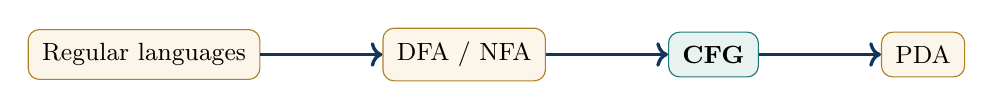
\begin{tikzpicture}[node distance=1.55cm]
    \node[note] (reg) {Regular languages};
    \node[note,right=of reg] (nfa) {DFA / NFA};
    \node[note,right=of nfa,draw=toccyan,fill=toccyan!10] (cfg) {\textbf{CFG}};
    \node[note,right=of cfg] (pda) {PDA};
    \draw[->,very thick,tocblue] (reg)--(nfa);
    \draw[->,very thick,tocblue] (nfa)--(cfg);
    \draw[->,very thick,tocblue] (cfg)--(pda);
\end{tikzpicture}

\vspace{1em}
Finite automata recognize patterns with finite memory.

\vspace{0.5em}
Context-free grammars generate strings with recursive, nested, or matched structure.

\begin{alertblock}{Guiding question}
How can a finite set of rules generate infinitely many structured strings?
\end{alertblock}
\end{frame}

% -------------------------------------------------
\begin{frame}{Learning Goals}
By the end of this lecture, you should be able to:

\begin{enumerate}
    \item define a context-free grammar formally;
    \item perform derivations using grammar rules;
    \item distinguish derivations, leftmost derivations, rightmost derivations, and parse trees;
    \item design CFGs for diverse recursive languages;
    \item identify and repair common ambiguity in grammars;
    \item simplify grammars by removing useless, nullable, and unit productions;
    \item convert a grammar to Chomsky Normal Form;
    \item run the CYK membership algorithm on a small example.
\end{enumerate}
\end{frame}

% =================================================
\section{Why Grammars?}
% =================================================

% -------------------------------------------------
\begin{frame}{From Recognition to Generation}
\small
A finite automaton asks:
\[
\boxed{\text{Is this string accepted?}}
\]

A grammar asks:
\[
\boxed{\text{How could this string be built?}}
\]

\vspace{0.5em}
\begin{columns}[T,onlytextwidth]
\column{0.48\textwidth}
\begin{block}{Recognizer view}
Read input from left to right and decide yes/no.
\end{block}

\column{0.48\textwidth}
\begin{exampleblock}{Generator view}
Start from a symbol and repeatedly expand it until only terminals remain.
\end{exampleblock}
\end{columns}

\vspace{0.8em}
The generator view is natural for syntax: programs, expressions, nested calls, trees, brackets, and protocols.
\end{frame}

% -------------------------------------------------
\begin{frame}{Recursive Objects Are Everywhere}
\small
\begin{columns}[T,onlytextwidth]
\column{0.32\textwidth}
\begin{block}{Nested brackets}
\[
\code{([]\{()\})}
\]
A valid object may contain smaller valid objects.
\end{block}

\column{0.32\textwidth}
\begin{exampleblock}{Function calls}
\[
\code{encrypt(hash(msg))}
\]
An argument may itself be a call.
\end{exampleblock}

\column{0.32\textwidth}
\begin{alertblock}{Mirrored packets}
\[
\code{101\#101}
\]
The second part checks the first part in reverse.
\end{alertblock}
\end{columns}

\vspace{1em}
All three examples require a rule like:
\[
\boxed{\text{a large valid object contains smaller valid objects}.}
\]
\end{frame}

% -------------------------------------------------
\begin{frame}{A Grammar Before the Definition}
\small
Consider properly nested parentheses:
\[
\eps,\quad (),\quad ()(),\quad (()),\quad (()()),\quad ((())())
\]

A compact set of construction rules is:
\[
S\to SS \mid (S) \mid \eps.
\]

\begin{columns}[T,onlytextwidth]
\column{0.32\textwidth}
\begin{block}{\(S\to\eps\)}
The empty string is balanced.
\end{block}

\column{0.32\textwidth}
\begin{exampleblock}{\(S\to(S)\)}
Wrapping a balanced string keeps it balanced.
\end{exampleblock}

\column{0.32\textwidth}
\begin{alertblock}{\(S\to SS\)}
Concatenating two balanced strings keeps it balanced.
\end{alertblock}
\end{columns}
\end{frame}

% -------------------------------------------------
\begin{frame}{Worked Derivation: Generating \( (()()) \)}
\small
Using
\[
S\to SS\mid (S)\mid\eps,
\]
we can derive:
\begin{align*}
S
&\der (S)\\
&\der (SS)\\
&\der ((S)S)\\
&\der (()S)\\
&\der (()(S))\\
&\der (()()).
\end{align*}

\begin{exampleblock}{Observation}
A derivation is a construction history. The same final string may sometimes have more than one construction history.
\end{exampleblock}
\end{frame}

% -------------------------------------------------
\begin{frame}{What a Grammar Is Good At}
\small
A grammar is good when strings can be built by repeatedly applying a few local construction principles.

\begin{center}
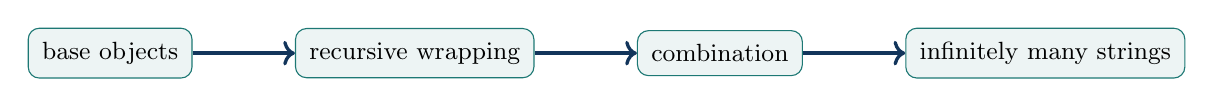
\begin{tikzpicture}[node distance=1.3cm]
    \node[syntax] (base) {base objects};
    \node[syntax,right=of base] (wrap) {recursive wrapping};
    \node[syntax,right=of wrap] (concat) {combination};
    \node[syntax,right=of concat] (all) {infinitely many strings};
    \draw[->,very thick,tocblue] (base)--(wrap);
    \draw[->,very thick,tocblue] (wrap)--(concat);
    \draw[->,very thick,tocblue] (concat)--(all);
\end{tikzpicture}
\end{center}

\vspace{0.5em}
\begin{alertblock}{Key intuition}
A CFG has only finitely many rules, but recursion lets those rules be reused arbitrarily many times.
\end{alertblock}
\end{frame}

% =================================================
\section{Formal Definition}
% =================================================

% -------------------------------------------------
\begin{frame}{Formal Definition of a CFG}
A context-free grammar is a 4-tuple
\[
G=(V,\Sigma,R,S),
\]
where:

\begin{itemize}
    \item \(V\) is a finite set of \alert{variables} or \alert{nonterminals};
    \item \(\Sigma\) is a finite set of \alert{terminals}, disjoint from \(V\);
    \item \(R\) is a finite set of productions;
    \item \(S\in V\) is the start variable.
\end{itemize}

\vspace{0.5em}
Each production has the form
\[
A\to \alpha,
\]
where \(A\in V\) and \(\alpha\in (V\cup\Sigma)^*\).
\end{frame}

% -------------------------------------------------
\begin{frame}{Variables Versus Terminals}
\small
\begin{columns}[T,onlytextwidth]
\column{0.48\textwidth}
\begin{block}{Variables}
Variables are placeholders for structured pieces not yet fully expanded.
\[
S,\quad E,\quad T,\quad Factor,\quad Stmt
\]
\end{block}

\column{0.48\textwidth}
\begin{exampleblock}{Terminals}
Terminals are the actual symbols that appear in the final string.
\[
0,1,+,*,(,),\code{if},\code{else}
\]
\end{exampleblock}
\end{columns}

\vspace{0.8em}
A derivation ends successfully only when no variables remain.
\[
S\ders w,
\qquad w\in\Sigma^*.
\]
\end{frame}

% -------------------------------------------------
\begin{frame}{Example Grammar as a 4-Tuple}
\small
For mixed brackets, let
\[
S\to SS\mid (S)\mid [S]\mid \{S\}\mid\eps.
\]

Then
\[
G_{br}=(V,\Sigma,R,S),
\]
where
\[
V=\{S\},
\]
\[
\Sigma=\{(,),[,],\{,\}\},
\]
and \(R\) is the set of five productions above.

\begin{exampleblock}{Language generated}
\[
L(G_{br})=\{w\mid w\text{ is a properly nested mixed-bracket string}\}.
\]
\end{exampleblock}
\end{frame}

% -------------------------------------------------
\begin{frame}{Reading Production Rules}
\small
A rule
\[
A\to \alpha
\]
means:

\begin{quote}
Whenever the current sentential form contains \(A\), we may replace that occurrence by \(\alpha\).
\end{quote}

\vspace{0.5em}
For example, if
\[
S\to 0S1\mid\#,
\]
then
\[
S\der 0S1\der 00S11\der 00\#11.
\]

\begin{alertblock}{Context-free means}
The rule for replacing \(A\) does not depend on the symbols around that occurrence of \(A\).
\end{alertblock}
\end{frame}

% -------------------------------------------------
\begin{frame}{Sentential Forms and Derivations}
\small
A \alert{sentential form} is any string over variables and terminals that can appear during a derivation.

\vspace{0.7em}
For the grammar
\[
S\to 0S1\mid\#,
\]
we have:
\[
S\der 0S1\der 00S11\der 00\#11.
\]

\begin{center}
\renewcommand{\arraystretch}{1.25}
\begin{tabular}{c|c}
Step & Sentential form\\
\hline
0 & \(S\)\\
1 & \(0S1\)\\
2 & \(00S11\)\\
3 & \(00\#11\)\\
\end{tabular}
\end{center}

The final line is a terminal string.
\end{frame}

% -------------------------------------------------
\begin{frame}{The Language of a Grammar}
\small
For a CFG \(G=(V,\Sigma,R,S)\), the language of \(G\) is
\[
L(G)=\{w\in\Sigma^*\mid S\ders w\}.
\]

\vspace{0.5em}
A language \(L\) is \alert{context-free} if there exists some CFG \(G\) such that
\[
L=L(G).
\]

\begin{exampleblock}{Important distinction}
A grammar is a description. A language is the set of strings described by the grammar.
\end{exampleblock}
\end{frame}

% =================================================
\section{Derivations}
% =================================================

% -------------------------------------------------
\begin{frame}{A Tiny Grammar for Nested Commands}
\small
Let us generate command strings such as
\[
\code{encrypt(sign(data))}.
\]

Use the grammar:
\[
\begin{aligned}
S&\to D\mid F(S),\\
F&\to \code{hash}\mid \code{sign}\mid \code{encrypt},\\
D&\to \code{data}\mid \code{msg}\mid \code{key}.
\end{aligned}
\]

\begin{block}{Interpretation}
A command is either raw data, or a function applied to a smaller command.
\end{block}
\end{frame}

% -------------------------------------------------
\begin{frame}{Worked Derivation: \code{encrypt(sign(data))}}
\small
\[
\begin{aligned}
S
&\der F(S)\\
&\der \code{encrypt}(S)\\
&\der \code{encrypt}(F(S))\\
&\der \code{encrypt}(\code{sign}(S))\\
&\der \code{encrypt}(\code{sign}(D))\\
&\der \code{encrypt}(\code{sign}(\code{data})).
\end{aligned}
\]

\begin{exampleblock}{What recursion did}
The outer command was generated first, but it forced the inside to be another valid command.
\end{exampleblock}
\end{frame}

% -------------------------------------------------
\begin{frame}{Leftmost and Rightmost Derivations}
\small
A sentential form may contain several variables.

\begin{block}{Leftmost derivation}
At each step, replace the leftmost variable.
\[
\der_{\mathrm{lm}}
\]
\end{block}

\begin{exampleblock}{Rightmost derivation}
At each step, replace the rightmost variable.
\[
\der_{\mathrm{rm}}
\]
\end{exampleblock}

\begin{alertblock}{Important}
Leftmost and rightmost derivations control the order of expansion. They do not necessarily change the final parse tree.
\end{alertblock}
\end{frame}

% -------------------------------------------------
\begin{frame}{Worked Leftmost Derivation}
\small
Use
\[
E\to E+T\mid T,
\quad
T\to T*F\mid F,
\quad
F\to (E)\mid a.
\]

A leftmost derivation of \(a+a*a\):
\begin{align*}
E
&\lmder E+T\\
&\lmder T+T\\
&\lmder F+T\\
&\lmder a+T\\
&\lmder a+T*F\\
&\lmder a+F*F\\
&\lmder a+a*F\\
&\lmder a+a*a.
\end{align*}
\end{frame}

% -------------------------------------------------
\begin{frame}{Worked Rightmost Derivation}
\small
Using the same grammar:
\begin{align*}
E
&\rmder E+T\\
&\rmder E+T*F\\
&\rmder E+T*a\\
&\rmder E+F*a\\
&\rmder E+a*a\\
&\rmder T+a*a\\
&\rmder F+a*a\\
&\rmder a+a*a.
\end{align*}

\begin{exampleblock}{Same string, same intended parse}
The expansion order changed, but the multiplication still binds inside the final \(T\).
\end{exampleblock}
\end{frame}

% -------------------------------------------------
\begin{frame}{Derivations Are Linear; Structure Is a Tree}
\small
A derivation is written as a sequence.

\[
E\der E+T\der T+T\der F+T\der a+T\der\cdots
\]

But the object being built is hierarchical.

\begin{center}
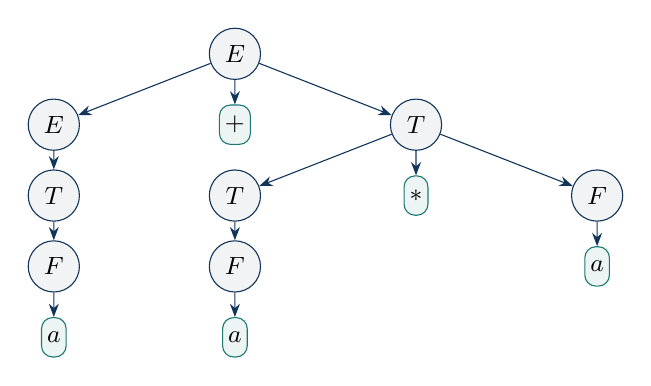
\begin{tikzpicture}[
level distance=9mm,
sibling distance=23mm,
every node/.style={font=\small},
edge from parent/.style={draw=tocblue,-Stealth}
]
\node[treevar] {$E$}
    child {node[treevar] {$E$}
        child {node[treevar] {$T$}
            child {node[treevar] {$F$}
                child {node[treeterm] {$a$}}}}}
    child {node[treeterm] {$+$}}
    child {node[treevar] {$T$}
        child {node[treevar] {$T$}
            child {node[treevar] {$F$}
                child {node[treeterm] {$a$}}}}
        child {node[treeterm] {$*$}}
        child {node[treevar] {$F$}
            child {node[treeterm] {$a$}}}};
\end{tikzpicture}
\end{center}
\end{frame}

% =================================================
\section{Parse Trees}
% =================================================

% -------------------------------------------------
\begin{frame}{Parse Trees: Formal Conditions}
\small
For a CFG \(G=(V,\Sigma,R,S)\), a parse tree satisfies:

\begin{enumerate}
    \item Each internal node is labeled by a variable.
    \item Each leaf is labeled by a variable, terminal, or \(\eps\).
    \item If an internal node labeled \(A\) has children labeled
    \[
    X_1,X_2,\ldots,X_k,
    \]
    then
    \[
    A\to X_1X_2\cdots X_k
    \]
    is a production.
\end{enumerate}

\begin{alertblock}{Special case}
If a leaf is labeled \(\eps\), it is the only child of its parent.
\end{alertblock}
\end{frame}

% -------------------------------------------------
\begin{frame}{Yield of a Parse Tree}
\small
The \alert{yield} of a parse tree is obtained by reading its leaves from left to right.

\begin{center}
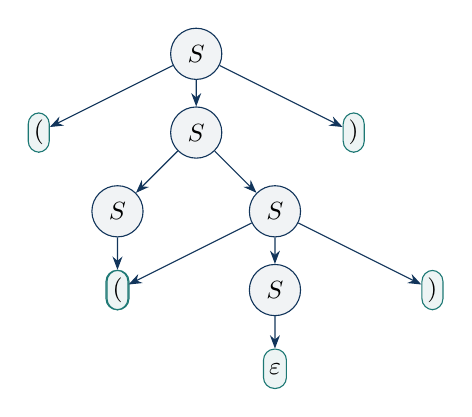
\begin{tikzpicture}[
level distance=10mm,
sibling distance=20mm,
edge from parent/.style={draw=tocblue,-Stealth}
]
\node[treevar] {$S$}
    child {node[treeterm] {$($}}
    child {node[treevar] {$S$}
        child {node[treevar] {$S$}
            child {node[treeterm] {$\eps$}}}
        child {node[treevar] {$S$}
            child {node[treeterm] {$($}}
            child {node[treevar] {$S$}
                child {node[treeterm] {$\eps$}}}
            child {node[treeterm] {$)$}}}}
    child {node[treeterm] {$)$}};
\end{tikzpicture}
\end{center}

\[
\text{yield}=\code{(())}
\]
\end{frame}

% -------------------------------------------------
\begin{frame}{Parse Tree for a Nested Command}
\small
\centering
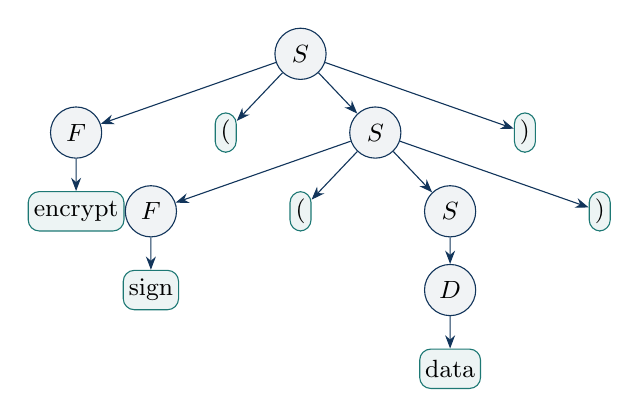
\begin{tikzpicture}[
level distance=10mm,
sibling distance=19mm,
edge from parent/.style={draw=tocblue,-Stealth}
]
\node[treevar] {$S$}
    child {node[treevar] {$F$}
        child {node[treeterm] {encrypt}}}
    child {node[treeterm] {$($}}
    child {node[treevar] {$S$}
        child {node[treevar] {$F$}
            child {node[treeterm] {sign}}}
        child {node[treeterm] {$($}}
        child {node[treevar] {$S$}
            child {node[treevar] {$D$}
                child {node[treeterm] {data}}}}
        child {node[treeterm] {$)$}}}
    child {node[treeterm] {$)$}};
\end{tikzpicture}

\vspace{0.7em}
\[
\text{yield}=\code{encrypt(sign(data))}
\]
\end{frame}

% -------------------------------------------------
\begin{frame}{Derivations and Parse Trees Are Equivalent}
\small
For every variable \(A\) and terminal string \(w\), the following are equivalent:

\begin{enumerate}
    \item \(A\ders w\).
    \item \(A\ders_{\mathrm{lm}} w\).
    \item \(A\ders_{\mathrm{rm}} w\).
    \item There is a parse tree with root \(A\) and yield \(w\).
\end{enumerate}

\begin{center}
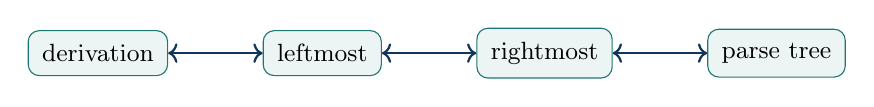
\begin{tikzpicture}[node distance=1.2cm]
    \node[syntax] (d) {derivation};
    \node[syntax,right=of d] (lm) {leftmost};
    \node[syntax,right=of lm] (rm) {rightmost};
    \node[syntax,right=of rm] (pt) {parse tree};
    \draw[<->,thick,tocblue] (d)--(lm);
    \draw[<->,thick,tocblue] (lm)--(rm);
    \draw[<->,thick,tocblue] (rm)--(pt);
\end{tikzpicture}
\end{center}

The proofs are by induction on derivation length or tree height.
\end{frame}

% -------------------------------------------------
\begin{frame}{Recursive Inference: Bottom-Up Thinking}
\small
Parse trees can be read top-down or bottom-up.

\begin{block}{Top-down}
Start from \(S\), expand variables, and try to generate the input.
\end{block}

\begin{exampleblock}{Bottom-up}
Start from small substrings and infer which variables could have generated them.
\end{exampleblock}

\vspace{0.5em}
The CYK algorithm at the end of the lecture is a systematic bottom-up parser for grammars in CNF.
\end{frame}

% =================================================
\section{Designing CFGs: Worked Examples}
% =================================================

% -------------------------------------------------
\begin{frame}{CFG Design Checklist}
\small
When designing a grammar, ask:

\begin{enumerate}
    \item What is the smallest valid string?
    \item How can a larger valid string be built from smaller valid strings?
    \item Is there a natural first/last pair to generate together?
    \item Is the language a union of simpler languages?
    \item Does part of the language happen to be regular?
    \item Which variables correspond to meaningful syntactic categories?
    \item Why can no invalid string be generated?
\end{enumerate}
\end{frame}

% -------------------------------------------------
\begin{frame}{Example 1: Balanced Mixed Brackets}
\small
\[
L_1=\{w\mid w\text{ is a properly nested string over }(),[],\{\}\}.
\]

\begin{exampleblock}{Grammar}
\[
S\to SS\mid (S)\mid [S]\mid \{S\}\mid\eps.
\]
\end{exampleblock}

\vspace{0.7em}
\begin{columns}[T,onlytextwidth]
\column{0.48\textwidth}
\begin{block}{Construction}
Wrap a balanced object, or concatenate two balanced objects.
\end{block}

\column{0.48\textwidth}
\begin{exampleblock}{Sample strings}
\[
\eps,\quad \code{()},\quad \code{([])},\quad \code{[]\{()\}}
\]
\end{exampleblock}
\end{columns}
\end{frame}

% -------------------------------------------------
\begin{frame}{Worked Derivation: \code{[]\{()\}}}
\small
\[
S\to SS\mid (S)\mid [S]\mid \{S\}\mid\eps.
\]

\begin{align*}
S
&\der SS\\
&\der [S]S\\
&\der []S\\
&\der []\{S\}\\
&\der []\{(S)\}\\
&\der []\{()\}.
\end{align*}

\begin{alertblock}{Rejection intuition}
Strings like \code{([)]} cannot be generated because every opening bracket must be closed by the matching wrapper rule.
\end{alertblock}
\end{frame}

% -------------------------------------------------
\begin{frame}{Why Example 1 Works}
\small
\begin{block}{Soundness}
Every rule preserves proper nesting:
\begin{itemize}
    \item \(\eps\) is balanced;
    \item \((S),[S],\{S\}\) wrap a balanced string with matching brackets;
    \item \(SS\) concatenates two balanced strings.
\end{itemize}
\end{block}

\begin{exampleblock}{Completeness}
Every nonempty balanced string is either:
\begin{itemize}
    \item one bracket pair surrounding a balanced inside; or
    \item a concatenation of two shorter balanced strings.
\end{itemize}
\end{exampleblock}
\end{frame}

% -------------------------------------------------
\begin{frame}{Example 2: Equal Numbers of 0s and 1s in Any Order}
\small
\[
L_2=\{w\in\{0,1\}^*\mid \#_0(w)=\#_1(w)\}.
\]

A grammar is:
\[
S\to 0S1S\mid 1S0S\mid\eps.
\]

\begin{block}{Why this is interesting}
The matching symbols need not be adjacent or appear in two blocks.
\[
\code{001011},\quad \code{0101},\quad \code{1010}\in L_2.
\]
\end{block}

\begin{alertblock}{Not merely \(0^n1^n\)}
This language allows arbitrary interleavings as long as the two counts agree.
\end{alertblock}
\end{frame}

% -------------------------------------------------
\begin{frame}{Worked Derivation: \code{0101}}
\small
Using
\[
S\to 0S1S\mid 1S0S\mid\eps,
\]
we derive:
\begin{align*}
S
&\der 0S1S\\
&\der 01S\\
&\der 010S1S\\
&\der 0101S\\
&\der 0101.
\end{align*}

\begin{exampleblock}{Invariant}
Each nonempty production introduces one \(0\) and one \(1\). Therefore every generated terminal string has equal counts.
\end{exampleblock}
\end{frame}

% -------------------------------------------------
\begin{frame}{Why the Grammar for Equal Counts Is Complete}
\small
Take a nonempty balanced string \(w\). Suppose it starts with \(0\).

\vspace{0.4em}
Scan from left to right until the first point where the number of \(0\)'s and \(1\)'s in the prefix becomes equal.

Then
\[
w=0x1y
\]
where \(x\) and \(y\) are both balanced.

\vspace{0.5em}
So the rule
\[
S\to 0S1S
\]
can generate it recursively.

\begin{alertblock}{Symmetric case}
If \(w\) starts with \(1\), use \(S\to 1S0S\).
\end{alertblock}
\end{frame}

% -------------------------------------------------
\begin{frame}{Example 3: Mirrored Packets}
\small
\[
L_3=\{w\#w^R\mid w\in\{0,1\}^*\}.
\]

\begin{exampleblock}{Grammar}
\[
S\to 0S0\mid 1S1\mid\#.
\]
\end{exampleblock}

\begin{block}{Construction}
Choose the middle marker \(\#\), then wrap equal symbols around it.
\end{block}

\begin{exampleblock}{Examples}
\[
\#,\quad 0\#0,
\quad 10\#01,
\quad 101\#101.
\]
\end{exampleblock}
\end{frame}

% -------------------------------------------------
\begin{frame}{Worked Derivation: \(101\#101\)}
\small
\begin{align*}
S
&\der 1S1\\
&\der 10S01\\
&\der 101S101\\
&\der 101\#101.
\end{align*}

\begin{center}
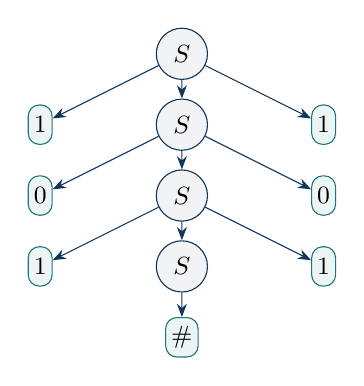
\begin{tikzpicture}[
level distance=9mm,
sibling distance=18mm,
edge from parent/.style={draw=tocblue,-Stealth}
]
\node[treevar] {$S$}
    child {node[treeterm] {$1$}}
    child {node[treevar] {$S$}
        child {node[treeterm] {$0$}}
        child {node[treevar] {$S$}
            child {node[treeterm] {$1$}}
            child {node[treevar] {$S$}
                child {node[treeterm] {$\#$}}}
            child {node[treeterm] {$1$}}}
        child {node[treeterm] {$0$}}}
    child {node[treeterm] {$1$}};
\end{tikzpicture}
\end{center}
\end{frame}

% -------------------------------------------------
\begin{frame}{Example 4: All Palindromes}
\small
\[
L_4=\{w\in\{0,1\}^*\mid w=w^R\}.
\]

\begin{exampleblock}{Grammar}
\[
P\to 0P0\mid 1P1\mid 0\mid 1\mid\eps.
\]
\end{exampleblock}

\vspace{0.5em}
\begin{columns}[T,onlytextwidth]
\column{0.48\textwidth}
\begin{block}{Even-length base}
\[
P\to\eps
\]
Examples: \(\eps,00,0110\).
\end{block}

\column{0.48\textwidth}
\begin{exampleblock}{Odd-length base}
\[
P\to0\mid1
\]
Examples: \(0,1,10101\).
\end{exampleblock}
\end{columns}
\end{frame}

% -------------------------------------------------
\begin{frame}{Example 5: Two Independent Matching Layers}
\small
\[
L_5=\{a^n b^m c^m d^n\mid n,m\ge0\}.
\]

\begin{exampleblock}{Grammar}
\[
S\to aSd\mid T,
\qquad
T\to bTc\mid\eps.
\]
\end{exampleblock}

\begin{block}{Idea}
The outer recursion matches \(a\)'s with \(d\)'s. The inner recursion matches \(b\)'s with \(c\)'s.
\end{block}

\[
\underbrace{a^n}_{S\text{ wraps}}
\underbrace{b^m c^m}_{T\text{ generates}}
\underbrace{d^n}_{S\text{ wraps}}
\]
\end{frame}

% -------------------------------------------------
\begin{frame}{Worked Derivation: \(a^2b^3c^3d^2\)}
\small
\begin{align*}
S
&\der aSd\\
&\der aaSdd\\
&\der aaTdd\\
&\der aabTcdd\\
&\der aabbTccdd\\
&\der aabbbTcccdd\\
&\der aabbbcccdd.
\end{align*}

\begin{exampleblock}{Design pattern}
Use one variable for each independent obligation, and nest variables when one equality must sit inside another.
\end{exampleblock}
\end{frame}

% -------------------------------------------------
\begin{frame}{Example 6: One of Two Equalities}
\small
\[
L_6=\{a^ib^jc^k\mid i=j\text{ or }j=k\}.
\]

Build the language as a union:
\[
S\to S_1\mid S_2.
\]

\begin{columns}[T,onlytextwidth]
\column{0.48\textwidth}
\begin{block}{Branch 1: verify \(i=j\)}
\[
S_1\to A C,
\quad
A\to aAb\mid\eps,
\quad
C\to cC\mid\eps.
\]
\end{block}

\column{0.48\textwidth}
\begin{exampleblock}{Branch 2: verify \(j=k\)}
\[
S_2\to D B,
\quad
D\to aD\mid\eps,
\quad
B\to bBc\mid\eps.
\]
\end{exampleblock}
\end{columns}
\end{frame}

% -------------------------------------------------
\begin{frame}{Example 7: Marked Middle Palindromes}
\small
\[
L_7=\{wcw^R\mid w\in\{a,b\}^*\}.
\]

\begin{exampleblock}{Grammar}
\[
S\to aSa\mid bSb\mid c.
\]
\end{exampleblock}

\begin{block}{Why the marker helps}
The symbol \(c\) explicitly marks the middle, so the grammar knows when to stop wrapping.
\end{block}

\begin{exampleblock}{Worked derivation}
\[
S\der aSa\der abSba\der abcba.
\]
\end{exampleblock}
\end{frame}

% -------------------------------------------------
\begin{frame}{Example 8: Binary Trees in Prefix Form}
\small
Let \(x\) be a leaf and \(n(T,T)\) be an internal node with two children.

\[
T\to x\mid n(T,T).
\]

\begin{columns}[T,onlytextwidth]
\column{0.45\textwidth}
\begin{exampleblock}{Generated strings}
\[
\code{x}
\]
\[
\code{n(x,x)}
\]
\[
\code{n(n(x,x),x)}
\]
\end{exampleblock}

\column{0.52\textwidth}
\centering
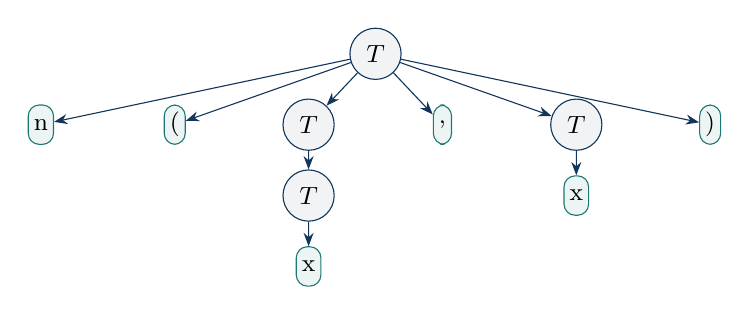
\begin{tikzpicture}[
level distance=9mm,
sibling distance=17mm,
edge from parent/.style={draw=tocblue,-Stealth}
]
\node[treevar] {$T$}
    child {node[treeterm] {n}}
    child {node[treeterm] {(}}
    child {node[treevar] {$T$}
        child {node[treevar] {$T$}
            child {node[treeterm] {x}}}}
    child {node[treeterm] {,}}
    child {node[treevar] {$T$}
        child {node[treeterm] {x}}}
    child {node[treeterm] {)}};
\end{tikzpicture}
\end{columns}
\end{frame}

% -------------------------------------------------
\begin{frame}{Example 9: A Tiny Query Language}
\small
Generate queries such as
\[
\code{select(name,where(age>18))}.
\]

\[
\begin{aligned}
Q&\to \code{select}(F,W),\\
F&\to \code{name}\mid\code{age}\mid\code{dept},\\
W&\to \code{all}\mid \code{where}(P),\\
P&\to F\ O\ V,\\
O&\to \code{>}\mid\code{=}\mid\code{<},\\
V&\to \code{18}\mid\code{30}\mid\code{cse}.
\end{aligned}
\]

\begin{block}{Moral}
Variables often represent syntactic categories, not just counting devices.
\end{block}
\end{frame}

% -------------------------------------------------
\begin{frame}{Worked Derivation: Query Language}
\small
\begin{align*}
Q
&\der \code{select}(F,W)\\
&\der \code{select}(\code{name},W)\\
&\der \code{select}(\code{name},\code{where}(P))\\
&\der \code{select}(\code{name},\code{where}(FOV))\\
&\der \code{select}(\code{name},\code{where}(\code{age}OV))\\
&\der \code{select}(\code{name},\code{where}(\code{age}>V))\\
&\der \code{select}(\code{name},\code{where}(\code{age}>\code{18})).
\end{align*}
\end{frame}

% -------------------------------------------------
\begin{frame}{Example 10: Converting a DFA to a CFG}
\small
Let
\[
L_{10}=\{w\in\{0,1\}^*\mid w\text{ contains the substring }101\}.
\]

\begin{center}
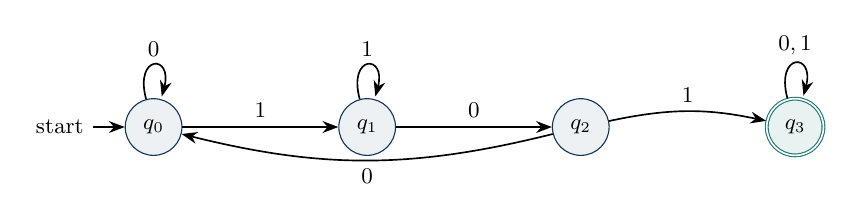
\begin{tikzpicture}[node distance=2.2cm,auto,scale=0.9,transform shape]
    \node[dfa,initial] (q0) {$q_0$};
    \node[dfa,right=of q0] (q1) {$q_1$};
    \node[dfa,right=of q1] (q2) {$q_2$};
    \node[acc,right=of q2] (q3) {$q_3$};
    \path
    (q0) edge[loop above] node {$0$} (q0)
    (q0) edge node {$1$} (q1)
    (q1) edge[loop above] node {$1$} (q1)
    (q1) edge node {$0$} (q2)
    (q2) edge[bend left=12] node[above] {$1$} (q3)
    (q2) edge[bend left=14] node[below] {$0$} (q0)
    (q3) edge[loop above] node {$0,1$} (q3);
\end{tikzpicture}
\end{center}

Make one variable \(R_i\) for each state \(q_i\).
\end{frame}

% -------------------------------------------------
\begin{frame}{DFA-to-CFG Construction}
\small
For every transition \(\delta(q_i,a)=q_j\), add
\[
R_i\to aR_j.
\]
For every accept state \(q_i\), add
\[
R_i\to\eps.
\]
The start variable is the variable corresponding to the DFA start state.

\vspace{0.7em}
For the substring \(101\) DFA:
\[
\begin{aligned}
R_0&\to 0R_0\mid 1R_1,\\
R_1&\to 1R_1\mid 0R_2,\\
R_2&\to 0R_0\mid 1R_3,\\
R_3&\to 0R_3\mid 1R_3\mid\eps.
\end{aligned}
\]
\end{frame}

% -------------------------------------------------
\begin{frame}{Example 11: A Tempting Non-Example}
\small
Consider
\[
L=\{ww\mid w\in\{0,1\}^*\}.
\]

Students often try:
\[
S\to 0S0\mid 1S1\mid\eps.
\]

But this generates
\[
\{ww^R\mid w\in\{0,1\}^*\},
\]
not \(\{ww\}\).

\begin{alertblock}{Important intuition}
Recursive wrapping remembers the first half in reverse order. This is exactly why stacks naturally recognize mirrors, not copies.
\end{alertblock}
\end{frame}

% -------------------------------------------------
\begin{frame}{Design Patterns We Have Used}
\small
\begin{center}
\renewcommand{\arraystretch}{1.35}
\begin{tabular}{p{0.32\textwidth}p{0.48\textwidth}}
\toprule
Pattern & Typical rule form\\
\midrule
Wrapping & \(S\to aSb\)\\
Concatenation & \(S\to SS\) or \(S\to AB\)\\
Optional structure & \(A\to \alpha\mid\eps\)\\
Union of cases & \(S\to S_1\mid S_2\)\\
Regular part & Convert DFA states into variables\\
Syntactic categories & One variable per category\\
\bottomrule
\end{tabular}
\end{center}
\end{frame}

% =================================================
\section{Ambiguity}
% =================================================

% -------------------------------------------------
\begin{frame}{Ambiguous Grammars}
\small
A string \(w\) is \alert{derived ambiguously} in a CFG \(G\) if it has two or more different parse trees.

Equivalently, it has:
\begin{itemize}
    \item two or more different leftmost derivations; or
    \item two or more different rightmost derivations.
\end{itemize}

\vspace{0.5em}
A grammar \(G\) is \alert{ambiguous} if it generates at least one string ambiguously.

\begin{alertblock}{Ambiguity is about grammar, not just language}
The same language may have both ambiguous and unambiguous grammars.
\end{alertblock}
\end{frame}

% -------------------------------------------------
\begin{frame}{Ambiguous Expression Grammar}
\small
Consider
\[
E\to E+E\mid E*E\mid (E)\mid a.
\]

The string
\[
\code{a+a*a}
\]
can be parsed as either
\[
\code{a+(a*a)}
\]
or
\[
\code{(a+a)*a}.
\]

\begin{alertblock}{Problem}
The grammar says that \(+\) and \(*\) are structurally equal, so it fails to encode precedence.
\end{alertblock}
\end{frame}

% -------------------------------------------------
\begin{frame}{Two Parse Trees for \(a+a*a\)}
\small
\begin{columns}[T,onlytextwidth]
\column{0.48\textwidth}
\centering
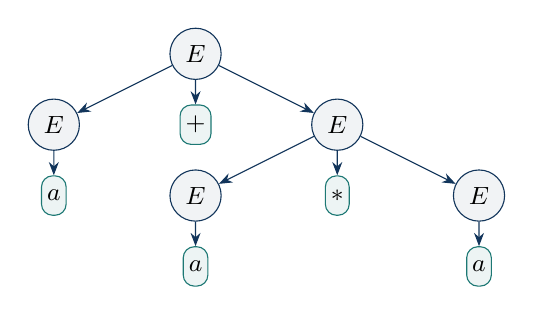
\begin{tikzpicture}[
level distance=9mm,
sibling distance=18mm,
edge from parent/.style={draw=tocblue,-Stealth}
]
\node[treevar] {$E$}
 child {node[treevar] {$E$} child {node[treeterm] {$a$}}}
 child {node[treeterm] {$+$}}
 child {node[treevar] {$E$}
    child {node[treevar] {$E$} child {node[treeterm] {$a$}}}
    child {node[treeterm] {$*$}}
    child {node[treevar] {$E$} child {node[treeterm] {$a$}}}};
\end{tikzpicture}

\[
a+(a*a)
\]

\column{0.48\textwidth}
\centering
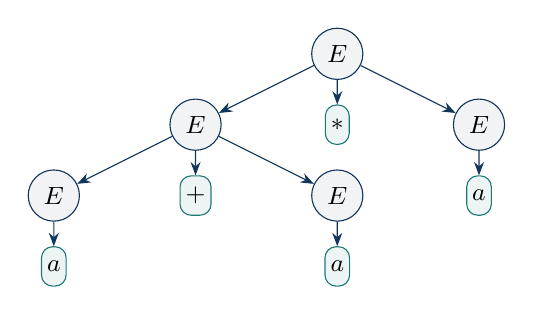
\begin{tikzpicture}[
level distance=9mm,
sibling distance=18mm,
edge from parent/.style={draw=tocblue,-Stealth}
]
\node[treevar] {$E$}
 child {node[treevar] {$E$}
    child {node[treevar] {$E$} child {node[treeterm] {$a$}}}
    child {node[treeterm] {$+$}}
    child {node[treevar] {$E$} child {node[treeterm] {$a$}}}}
 child {node[treeterm] {$*$}}
 child {node[treevar] {$E$} child {node[treeterm] {$a$}}};
\end{tikzpicture}

\[
(a+a)*a
\]
\end{columns}
\end{frame}

% -------------------------------------------------
\begin{frame}{Removing Expression Ambiguity}
\small
We introduce levels:

\begin{itemize}
    \item \(F\): factor, cannot be split by an adjacent operator;
    \item \(T\): term, product of factors;
    \item \(E\): expression, sum of terms.
\end{itemize}

\[
\begin{aligned}
E&\to E+T\mid T,\\
T&\to T*F\mid F,\\
F&\to (E)\mid a.
\end{aligned}
\]

\begin{exampleblock}{Result}
Multiplication is forced below addition in the tree, so \(*\) binds more tightly than \(+\).
\end{exampleblock}
\end{frame}

% -------------------------------------------------
\begin{frame}{Parse Tree After Removing Ambiguity}
\small
\centering
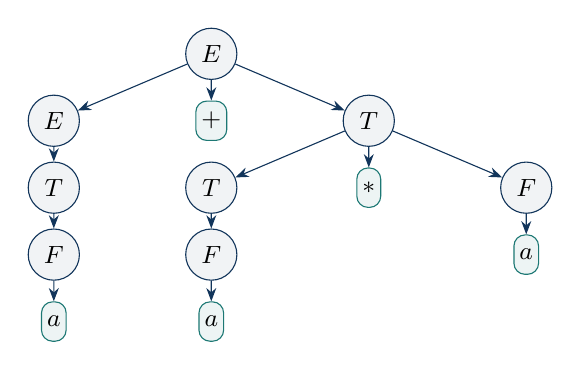
\begin{tikzpicture}[
level distance=8.5mm,
sibling distance=20mm,
edge from parent/.style={draw=tocblue,-Stealth}
]
\node[treevar] {$E$}
    child {node[treevar] {$E$}
        child {node[treevar] {$T$}
            child {node[treevar] {$F$}
                child {node[treeterm] {$a$}}}}}
    child {node[treeterm] {$+$}}
    child {node[treevar] {$T$}
        child {node[treevar] {$T$}
            child {node[treevar] {$F$}
                child {node[treeterm] {$a$}}}}
        child {node[treeterm] {$*$}}
        child {node[treevar] {$F$}
            child {node[treeterm] {$a$}}}};
\end{tikzpicture}

\vspace{0.5em}
\[
\code{a+a*a}\quad\text{is forced to mean}\quad \code{a+(a*a)}.
\]
\end{frame}

% -------------------------------------------------
\begin{frame}{Ambiguity Example: Dangling Else}
\small
A naive statement grammar:
\[
S\to \code{if }E\code{ then }S
\mid \code{if }E\code{ then }S\code{ else }S
\mid \code{other}.
\]

The string
\[
\code{if E then if E then other else other}
\]
can attach \code{else} to:

\begin{columns}[T,onlytextwidth]
\column{0.48\textwidth}
\begin{block}{Inner if}
\[
\code{if E then (if E then other else other)}
\]
\end{block}

\column{0.48\textwidth}
\begin{alertblock}{Outer if}
\[
\code{if E then (if E then other) else other}
\]
\end{alertblock}
\end{columns}
\end{frame}

% -------------------------------------------------
\begin{frame}{Repairing Dangling Else}
\small
Separate matched and unmatched statements.

\[
\begin{aligned}
S&\to M\mid U,\\
M&\to \code{other}\mid \code{if }E\code{ then }M\code{ else }M,\\
U&\to \code{if }E\code{ then }S
\mid \code{if }E\code{ then }M\code{ else }U.
\end{aligned}
\]

\begin{exampleblock}{Convention encoded}
Every \code{else} attaches to the nearest unmatched \code{if}.
\end{exampleblock}
\end{frame}

% -------------------------------------------------
\begin{frame}{Structural Ambiguity in Balanced Parentheses}
\small
The grammar
\[
S\to SS\mid(S)\mid\eps
\]
correctly generates balanced parentheses, but it is ambiguous.

For example:
\[
\code{()()()}
\]
can be grouped as
\[
(\code{()}\ \code{()})\ \code{()}
\]
or as
\[
\code{()}\ (\code{()}\ \code{()}).
\]

\begin{alertblock}{Lesson}
A language may have an obvious structure, but a grammar may still give multiple parse trees for concatenation.
\end{alertblock}
\end{frame}

% -------------------------------------------------
\begin{frame}{Inherent Ambiguity}
\small
A CFL \(L\) is \alert{inherently ambiguous} if every CFG for \(L\) is ambiguous.

A standard example is:
\[
\begin{aligned}
L={}&\{a^n b^n c^m d^m\mid n,m\ge1\}\\
&\cup\{a^n b^m c^m d^n\mid n,m\ge1\}.
\end{aligned}
\]

\begin{block}{Why ambiguity is unavoidable}
Strings of the form
\[
a^n b^n c^n d^n
\]
belong to both sides of the union.
\end{block}
\end{frame}

% -------------------------------------------------
\begin{frame}{Grammar for the Inherently Ambiguous Example}
\small
\[
\begin{aligned}
S&\to AB\mid C,\\
A&\to aAb\mid ab,\\
B&\to cBd\mid cd,\\
C&\to aCd\mid aDd,\\
D&\to bDc\mid bc.
\end{aligned}
\]

\begin{columns}[T,onlytextwidth]
\column{0.48\textwidth}
\begin{block}{Branch \(AB\)}
Matches \(a\)'s with \(b\)'s and \(c\)'s with \(d\)'s.
\end{block}

\column{0.48\textwidth}
\begin{exampleblock}{Branch \(C\)}
Matches outer \(a,d\) and inner \(b,c\).
\end{exampleblock}
\end{columns}
\end{frame}

% =================================================
\section{Simplifying Grammars}
% =================================================

% -------------------------------------------------
\begin{frame}{Why Simplify Grammars?}
\small
Before converting to normal forms or running parsing algorithms, we clean up grammar rules.

\begin{center}
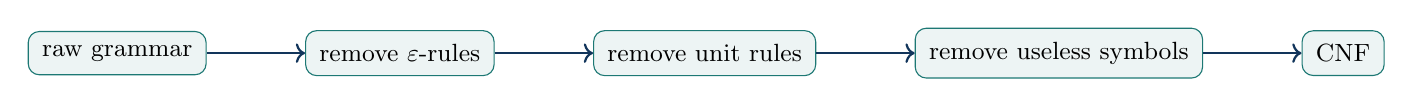
\begin{tikzpicture}[node distance=1.25cm]
    \node[syntax] (g) {raw grammar};
    \node[syntax,right=of g] (e) {remove \(\eps\)-rules};
    \node[syntax,right=of e] (u) {remove unit rules};
    \node[syntax,right=of u] (x) {remove useless symbols};
    \node[syntax,right=of x] (cnf) {CNF};
    \draw[->,thick,tocblue] (g)--(e);
    \draw[->,thick,tocblue] (e)--(u);
    \draw[->,thick,tocblue] (u)--(x);
    \draw[->,thick,tocblue] (x)--(cnf);
\end{tikzpicture}
\end{center}

\begin{alertblock}{Goal}
Keep the same language while removing grammar clutter that complicates algorithms.
\end{alertblock}
\end{frame}

% -------------------------------------------------
\begin{frame}{Useless Symbols}
\small
A symbol is \alert{useful} if it is both:

\begin{enumerate}
    \item \alert{generating}: it can derive some terminal string;
    \item \alert{reachable}: it can appear in some derivation from the start symbol.
\end{enumerate}

\[
\text{useful}=\text{generating}+\text{reachable}.
\]

\begin{columns}[T,onlytextwidth]
\column{0.48\textwidth}
\begin{block}{Generating}
\[
X\ders w\quad\text{for some }w\in\Sigma^*.
\]
\end{block}

\column{0.48\textwidth}
\begin{exampleblock}{Reachable}
\[
S\ders \alpha X\beta.
\]
\end{exampleblock}
\end{columns}
\end{frame}

% -------------------------------------------------
\begin{frame}{Worked Example: Useless Symbols}
\small
Consider
\[
\begin{aligned}
S&\to AB\mid a,\\
A&\to b,\\
B&\to CD,\\
C&\to c,\\
D&\to DE,\\
E&\to e,\\
F&\to f.
\end{aligned}
\]

\begin{columns}[T,onlytextwidth]
\column{0.48\textwidth}
\begin{block}{Generating symbols}
\[
A,C,E,F,S
\]
\(D\) is not generating, so \(B\) is not generating.
\end{block}

\column{0.48\textwidth}
\begin{alertblock}{Reachable symbols}
\[
S,A,B,C,D,E
\]
\(F\) is generating but unreachable.
\end{alertblock}
\end{columns}
\end{frame}

% -------------------------------------------------
\begin{frame}{Removing Useless Symbols}
\small
From the grammar
\[
\begin{aligned}
S&\to AB\mid a,\quad A\to b,\quad B\to CD,\quad C\to c,\\
D&\to DE,\quad E\to e,\quad F\to f,
\end{aligned}
\]
remove symbols that are not both generating and reachable.

\vspace{0.5em}
\begin{block}{Result}
\[
S\to a,
\qquad
A\to b.
\]
But after removing unreachable symbols again, only
\[
S\to a
\]
remains.
\end{block}

\begin{alertblock}{Reason}
The branch \(S\to AB\) can never terminate because \(B\) cannot generate a terminal string.
\end{alertblock}
\end{frame}

% -------------------------------------------------
\begin{frame}{Nullable Variables and \(\eps\)-Productions}
\small
A variable \(A\) is \alert{nullable} if
\[
A\ders\eps.
\]

If \(A\) is nullable and appears in a production body, then that occurrence may be kept or omitted.

\vspace{0.5em}
Example:
\[
B\to C A D
\]
with \(A\) nullable gives both
\[
B\to C A D
\qquad\text{and}\qquad
B\to C D.
\]

\begin{alertblock}{If several nullable occurrences appear}
Generate all omission patterns, then remove duplicates and forbidden empty bodies unless the start variable must keep \(\eps\).
\end{alertblock}
\end{frame}

% -------------------------------------------------
\begin{frame}{Worked Example: Eliminating \(\eps\)-Productions}
\small
Consider optional query filters:
\[
\begin{aligned}
S&\to \code{select}(F,W),\\
W&\to \code{where}(P)\mid\eps,\\
F&\to \code{name}\mid\code{age},\\
P&\to F\code{>}\code{18}.
\end{aligned}
\]

Here \(W\) is nullable.

So the rule
\[
S\to \code{select}(F,W)
\]
becomes
\[
S\to \code{select}(F,W)
\mid
\code{select}(F,).
\]

\begin{alertblock}{Engineering note}
Real languages often design syntax to avoid ugly leftover punctuation when optional parts disappear.
\end{alertblock}
\end{frame}

% -------------------------------------------------
\begin{frame}{A Cleaner Optional-Filter Grammar}
\small
Better grammar:
\[
\begin{aligned}
S&\to \code{select}(F)\mid \code{select}(F,W),\\
W&\to \code{where}(P),\\
F&\to \code{name}\mid\code{age},\\
P&\to F\code{>}\code{18}.
\end{aligned}
\]

\begin{exampleblock}{Lesson}
Grammar design choices affect both syntax quality and later simplification steps.
\end{exampleblock}
\end{frame}

% -------------------------------------------------
\begin{frame}{Unit Productions}
\small
A \alert{unit production} has the form
\[
A\to B,
\]
where both \(A\) and \(B\) are variables.

Unit productions are often alias or forwarding rules:
\[
E\to T,
\qquad
T\to F,
\qquad
F\to I.
\]

\begin{block}{Elimination idea}
If \(A\ders B\) using only unit productions, then \(A\) should inherit every nonunit production of \(B\).
\end{block}
\end{frame}

% -------------------------------------------------
\begin{frame}{Worked Unit-Pair Closure}
\small
Consider
\[
E\to T\mid E+T,
\quad
T\to F\mid T*F,
\quad
F\to I\mid(E),
\quad
I\to a\mid b.
\]

Unit pairs include:
\[
(E,E),(E,T),(E,F),(E,I),
\]
\[
(T,T),(T,F),(T,I),
\]
\[
(F,F),(F,I),(I,I).
\]

\begin{exampleblock}{Example inheritance}
Because \((E,I)\) is a unit pair and \(I\to a\mid b\), add
\[
E\to a\mid b.
\]
\end{exampleblock}
\end{frame}

% -------------------------------------------------
\begin{frame}{After Removing Unit Productions}
\small
From the previous grammar, the nonunit productions inherited by each variable are:

\[
\begin{aligned}
E&\to E+T\mid T*F\mid(E)\mid a\mid b,\\
T&\to T*F\mid(E)\mid a\mid b,\\
F&\to (E)\mid a\mid b,\\
I&\to a\mid b.
\end{aligned}
\]

\begin{alertblock}{Then delete the unit rules}
Rules such as \(E\to T\), \(T\to F\), and \(F\to I\) are no longer needed.
\end{alertblock}
\end{frame}

% =================================================
\section{Chomsky Normal Form}
% =================================================

% -------------------------------------------------
\begin{frame}{Chomsky Normal Form}
\small
A grammar is in \alert{Chomsky Normal Form} if every production has one of the forms:
\[
A\to BC,
\qquad
A\to a,
\]
where \(A,B,C\) are variables and \(a\) is a terminal.

If the language contains \(\eps\), we also allow the start rule
\[
S_0\to\eps,
\]
provided \(S_0\) does not appear on the right-hand side.

\begin{exampleblock}{Theorem}
Every context-free language has an equivalent grammar in Chomsky Normal Form.
\end{exampleblock}
\end{frame}

% -------------------------------------------------
\begin{frame}{Why CNF Matters}
\small
CNF is not designed for human readability.

\vspace{0.5em}
It is designed for algorithms and proofs.

\begin{columns}[T,onlytextwidth]
\column{0.48\textwidth}
\begin{block}{Uniform parse trees}
Every internal node has exactly two children, except terminal leaves.
\end{block}

\column{0.48\textwidth}
\begin{exampleblock}{Dynamic programming}
CYK can combine two smaller substrings using one rule
\[
A\to BC.
\]
\end{exampleblock}
\end{columns}
\end{frame}

% -------------------------------------------------
\begin{frame}{CNF Conversion Pipeline}
\small
\begin{center}
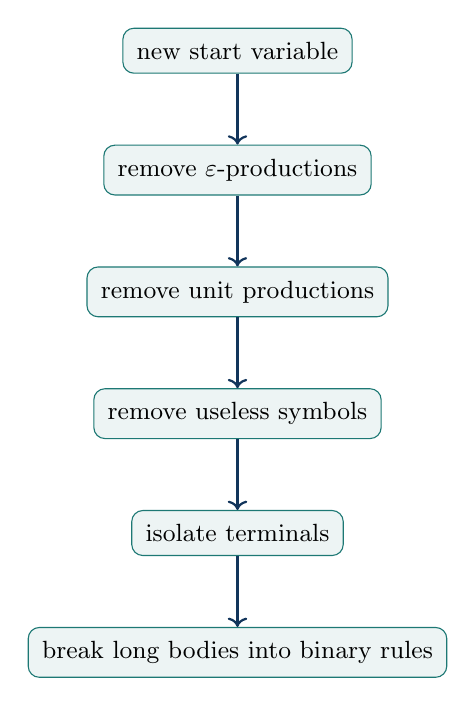
\begin{tikzpicture}[node distance=0.9cm]
\node[syntax] (s0) {new start variable};
\node[syntax,below=of s0] (eps) {remove \(\eps\)-productions};
\node[syntax,below=of eps] (unit) {remove unit productions};
\node[syntax,below=of unit] (useless) {remove useless symbols};
\node[syntax,below=of useless] (term) {isolate terminals};
\node[syntax,below=of term] (bin) {break long bodies into binary rules};
\draw[->,thick,tocblue] (s0)--(eps);
\draw[->,thick,tocblue] (eps)--(unit);
\draw[->,thick,tocblue] (unit)--(useless);
\draw[->,thick,tocblue] (useless)--(term);
\draw[->,thick,tocblue] (term)--(bin);
\end{tikzpicture}
\end{center}
\end{frame}

% -------------------------------------------------
\begin{frame}{CNF Worked Example: Starting Grammar}
\small
Use a small list grammar:
\[
\begin{aligned}
S&\to [L],\\
L&\to I\mid I,L\mid\eps,\\
I&\to a\mid b.
\end{aligned}
\]

It generates strings like:
\[
\code{[]},\quad \code{[a]},\quad \code{[a,b]},\quad \code{[b,a,a]}.
\]

\begin{alertblock}{Problems for CNF}
There is an \(\eps\)-production, unit production, terminals in long bodies, and bodies longer than two.
\end{alertblock}
\end{frame}

% -------------------------------------------------
\begin{frame}{Step 1: Add a New Start Variable}
\small
Create
\[
S_0\to S.
\]

Now the grammar is:
\[
\begin{aligned}
S_0&\to S,\\
S&\to [L],\\
L&\to I\mid I,L\mid\eps,\\
I&\to a\mid b.
\end{aligned}
\]

\begin{exampleblock}{Why?}
The new start variable protects the original start symbol during later transformations, especially when \(\eps\) is involved.
\end{exampleblock}
\end{frame}

% -------------------------------------------------
\begin{frame}{Step 2: Remove \(\eps\)-Production}
\small
The nullable variable is \(L\). Since
\[
S\to [L]
\]
contains nullable \(L\), add the version where \(L\) is omitted:
\[
S\to [] .
\]

Remove \(L\to\eps\):
\[
\begin{aligned}
S_0&\to S,\\
S&\to [L]\mid [],\\
L&\to I\mid I,L,\\
I&\to a\mid b.
\end{aligned}
\]

\begin{alertblock}{The language still contains \(\code{[]}\)}
It is now generated by \(S\to []\), not by \(L\to\eps\).
\end{alertblock}
\end{frame}

% -------------------------------------------------
\begin{frame}{Step 3: Remove Unit Productions}
\small
Unit productions:
\[
S_0\to S,
\qquad
L\to I.
\]

Inherit nonunit productions:
\[
\begin{aligned}
S_0&\to [L]\mid [],\\
S&\to [L]\mid [],\\
L&\to I,L\mid a\mid b,\\
I&\to a\mid b.
\end{aligned}
\]

Now remove useless symbols if desired. Since \(S
ot\) reachable from \(S_0\) anymore, remove \(S\):
\[
\begin{aligned}
S_0&\to [L]\mid [],\\
L&\to I,L\mid a\mid b,\\
I&\to a\mid b.
\end{aligned}
\]
\end{frame}

% -------------------------------------------------
\begin{frame}{Step 4: Isolate Terminals in Long Bodies}
\small
Introduce variables for terminals that appear in longer bodies:
\[
A\to a,
\quad
B\to b,
\quad
LB\to [,
\quad
RB\to ],
\quad
C\to ,.
\]

Replace terminals inside longer bodies:
\[
\begin{aligned}
S_0&\to LB\ L\ RB\mid LB\ RB,\\
L&\to I\ C\ L\mid a\mid b,\\
I&\to a\mid b,\\
LB&\to [,\qquad RB\to ],\qquad C\to ,.
\end{aligned}
\]

\begin{alertblock}{Single-terminal rules are already CNF}
Rules like \(L\to a\) and \(I\to b\) are allowed.
\end{alertblock}
\end{frame}

% -------------------------------------------------
\begin{frame}{Step 5: Break Long Bodies into Binary Rules}
\small
Break
\[
S_0\to LB\ L\ RB
\]
using
\[
X_1\to L\ RB,
\qquad
S_0\to LB\ X_1.
\]

Break
\[
L\to I\ C\ L
\]
using
\[
X_2\to C\ L,
\qquad
L\to I\ X_2.
\]

Final CNF-style grammar:
\[
\begin{aligned}
S_0&\to LB\ X_1\mid LB\ RB,\\
X_1&\to L\ RB,\\
L&\to I\ X_2\mid a\mid b,\\
X_2&\to C\ L,\\
I&\to a\mid b,\\
LB&\to [,\quad RB\to ],\quad C\to ,.
\end{aligned}
\]
\end{frame}

% =================================================
\section{CYK Membership Testing}
% =================================================

% -------------------------------------------------
\begin{frame}{CYK: Membership Testing for CFLs}
\small
Given:
\begin{itemize}
    \item a grammar \(G\) in CNF;
    \item an input string \(w=a_1a_2\cdots a_n\).
\end{itemize}

CYK builds a triangular dynamic-programming table.

\vspace{0.5em}
Entry \(X_{ij}\) contains all variables \(A\) such that
\[
A\ders a_i a_{i+1}\cdots a_j.
\]

\begin{alertblock}{Acceptance criterion}
\[
w\in L(G)\quad\Longleftrightarrow\quad S\in X_{1n}.
\]
\end{alertblock}
\end{frame}

% -------------------------------------------------
\begin{frame}{CYK Recurrence}
\small
Base case:
\[
A\in X_{ii}
\quad\text{if}\quad
A\to a_i.
\]

For \(i<j\), include \(A\in X_{ij}\) if there exists \(k\) with
\[
i\le k<j,
\]
and variables \(B,C\) such that
\[
B\in X_{ik},
\qquad
C\in X_{k+1,j},
\qquad
A\to BC.
\]

\begin{exampleblock}{Meaning}
Try every split of the substring, and see whether a CNF rule combines the two halves.
\end{exampleblock}
\end{frame}

% -------------------------------------------------
\begin{frame}{CYK Worked Example: Grammar}
\small
Use the CNF grammar for \(\{a^n b^n\mid n\ge1\}\):
\[
\begin{aligned}
S&\to AB\mid AT,\\
T&\to SB,\\
A&\to a,\\
B&\to b.
\end{aligned}
\]

Test the string
\[
w=\code{aabb}.
\]

\begin{block}{Goal}
We will determine whether \(S\in X_{14}\).
\end{block}
\end{frame}

% -------------------------------------------------
\begin{frame}{CYK Table: Base Row}
\small
\[
w=a_1a_2a_3a_4=\code{aabb}.
\]

\begin{center}
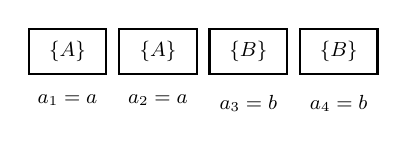
\begin{tikzpicture}[scale=0.82,transform shape]
\foreach \i/\lab in {1/a,2/a,3/b,4/b}{
    \node[below] at (\i*1.4,0) {$a_{\i}=\lab$};
}
\foreach \i/\txt in {1/\{A\},2/\{A\},3/\{B\},4/\{B\}}{
    \draw[thick] (\i*1.4-0.6,0.2) rectangle (\i*1.4+0.6,0.9);
    \node at (\i*1.4,0.55) {$\txt$};
}
\end{tikzpicture}
\end{center}

\begin{exampleblock}{Reason}
\[
A\to a,
\qquad
B\to b.
\]
So each one-letter cell receives the variable that generates that terminal.
\end{exampleblock}
\end{frame}

% -------------------------------------------------
\begin{frame}{CYK Table: Length 2 Substrings}
\small
Substrings of length 2:
\[
\code{aa},\quad \code{ab},\quad \code{bb}.
\]

Only \(\code{ab}\) can be generated by \(S\), because
\[
S\to AB,
\quad A\in X_{22},
\quad B\in X_{33}.
\]

\begin{center}
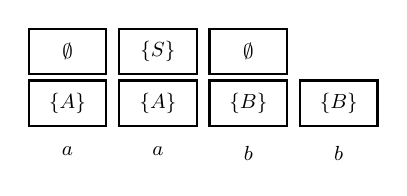
\begin{tikzpicture}[scale=0.82,transform shape]
\foreach \i/\txt in {1/\{A\},2/\{A\},3/\{B\},4/\{B\}}{
    \draw[thick] (\i*1.4-0.6,0.2) rectangle (\i*1.4+0.6,0.9);
    \node at (\i*1.4,0.55) {$\txt$};
}
\foreach \i/\txt in {1/\emptyset,2/\{S\},3/\emptyset}{
    \draw[thick] (\i*1.4-0.6,1.0) rectangle (\i*1.4+0.6,1.7);
    \node at (\i*1.4,1.35) {$\txt$};
}
\node[below] at (1.4,0) {$a$}; \node[below] at (2.8,0) {$a$};
\node[below] at (4.2,0) {$b$}; \node[below] at (5.6,0) {$b$};
\end{tikzpicture}
\end{center}
\end{frame}

% -------------------------------------------------
\begin{frame}{CYK Table: Length 3 Substrings}
\small
For substring \(\code{abb}\), we have:
\[
X_{23}=\{S\},
\qquad
X_{44}=\{B\},
\qquad
T\to SB.
\]

Therefore
\[
T\in X_{24}.
\]

\begin{center}
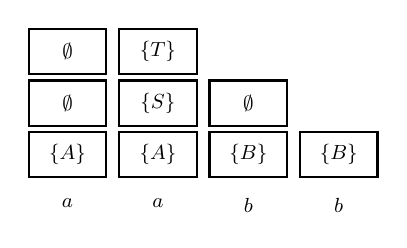
\begin{tikzpicture}[scale=0.82,transform shape]
\foreach \i/\txt in {1/\{A\},2/\{A\},3/\{B\},4/\{B\}}{
    \draw[thick] (\i*1.4-0.6,0.2) rectangle (\i*1.4+0.6,0.9);
    \node at (\i*1.4,0.55) {$\txt$};
}
\foreach \i/\txt in {1/\emptyset,2/\{S\},3/\emptyset}{
    \draw[thick] (\i*1.4-0.6,1.0) rectangle (\i*1.4+0.6,1.7);
    \node at (\i*1.4,1.35) {$\txt$};
}
\foreach \i/\txt in {1/\emptyset,2/\{T\}}{
    \draw[thick] (\i*1.4-0.6,1.8) rectangle (\i*1.4+0.6,2.5);
    \node at (\i*1.4,2.15) {$\txt$};
}
\node[below] at (1.4,0) {$a$}; \node[below] at (2.8,0) {$a$};
\node[below] at (4.2,0) {$b$}; \node[below] at (5.6,0) {$b$};
\end{tikzpicture}
\end{center}
\end{frame}

% -------------------------------------------------
\begin{frame}{CYK Table: Final Cell}
\small
For the full string \(\code{aabb}\):
\[
X_{11}=\{A\},
\qquad
X_{24}=\{T\},
\qquad
S\to AT.
\]

Therefore
\[
S\in X_{14}.
\]

\begin{center}
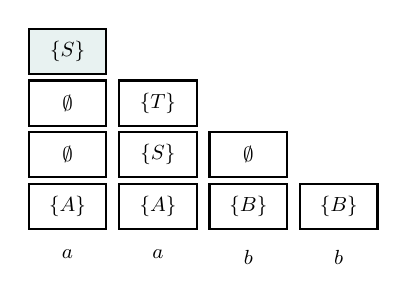
\begin{tikzpicture}[scale=0.82,transform shape]
\foreach \i/\txt in {1/\{A\},2/\{A\},3/\{B\},4/\{B\}}{
    \draw[thick] (\i*1.4-0.6,0.2) rectangle (\i*1.4+0.6,0.9);
    \node at (\i*1.4,0.55) {$\txt$};
}
\foreach \i/\txt in {1/\emptyset,2/\{S\},3/\emptyset}{
    \draw[thick] (\i*1.4-0.6,1.0) rectangle (\i*1.4+0.6,1.7);
    \node at (\i*1.4,1.35) {$\txt$};
}
\foreach \i/\txt in {1/\emptyset,2/\{T\}}{
    \draw[thick] (\i*1.4-0.6,1.8) rectangle (\i*1.4+0.6,2.5);
    \node at (\i*1.4,2.15) {$\txt$};
}
\draw[thick,fill=toccyan!10] (1.4-0.6,2.6) rectangle (1.4+0.6,3.3);
\node at (1.4,2.95) {$\{S\}$};
\node[below] at (1.4,0) {$a$}; \node[below] at (2.8,0) {$a$};
\node[below] at (4.2,0) {$b$}; \node[below] at (5.6,0) {$b$};
\end{tikzpicture}
\end{center}

Since \(S\in X_{14}\), CYK accepts \(\code{aabb}\).
\end{frame}

% -------------------------------------------------
\begin{frame}{Why CYK Runs in \(O(n^3)\)}
\small
There are \(O(n^2)\) table cells.

For each cell \(X_{ij}\), we try \(O(n)\) split positions:
\[
i\le k<j.
\]

For each split, we check whether some rule
\[
A\to BC
\]
combines variables from the left and right cells.

\begin{exampleblock}{Main bound}
With the grammar fixed, the running time is
\[
O(n^3).
\]
\end{exampleblock}
\end{frame}

% =================================================
\section{Recap and Bridge to PDA}
% =================================================

% -------------------------------------------------
\begin{frame}{Today's Big Picture}
\small
\begin{center}
\Large
\textbf{CFGs describe recursive construction.}
\end{center}

\vspace{0.8em}
\begin{columns}[T,onlytextwidth]
\column{0.32\textwidth}
\begin{block}{Rules}
A finite set of productions expands variables into structure.
\end{block}

\column{0.32\textwidth}
\begin{exampleblock}{Trees}
Parse trees reveal the hierarchy hidden inside the string.
\end{exampleblock}

\column{0.32\textwidth}
\begin{alertblock}{Algorithms}
CNF and CYK turn grammar membership into dynamic programming.
\end{alertblock}
\end{columns}
\end{frame}

% -------------------------------------------------
\begin{frame}{Practice Problems}
\small
Design CFGs for the following languages.

\begin{enumerate}
    \item \(\{a^n b^m c^n\mid n,m\ge0\}\)
    \item \(\{w\#x\mid w,x\in\{0,1\}^*,\ |w|=|x|\}\)
    \item Properly nested XML-like tags using only \(\code{<a>}\) and \(\code{</a>}\).
    \item Boolean formulas over \(p,q\) using \(\neg,\land,\lor\), with standard precedence.
    \item \(\{w\in\{0,1\}^*\mid w\text{ has equal numbers of }01\text{ and }10\}\).
\end{enumerate}

\begin{alertblock}{Challenge}
For each grammar, state why invalid strings cannot be generated.
\end{alertblock}
\end{frame}

% -------------------------------------------------
\begin{frame}{Bridge to Pushdown Automata}
\small
A CFG tells us how a string may be generated.

\vspace{0.7em}
The next question is:
\[
\boxed{\text{Can a machine recognize exactly the strings generated by a CFG?}}
\]

\vspace{0.7em}
The answer is yes.

\begin{exampleblock}{Next model}
A pushdown automaton is a finite automaton equipped with one unbounded stack.
\end{exampleblock}

\vspace{0.5em}
The stack will remember exactly the kind of nested and matched structure that CFGs generate.
\end{frame}

\end{document}
